\documentclass[preprint]{aastex}  
%\documentclass[iop]{emulateapj}
%\usepackage{booktabs,caption,fixltx2e}
\usepackage{natbib}
\bibliographystyle{aa}

\usepackage{graphicx,color,rotating}
\usepackage{footnote,lineno}
\usepackage{ulem} 
\usepackage{xspace}
%\linenumbers
%%%%%%%%%%%%%%%%%%%%%%%%%%%%%%%%%%%%%%%%
%\usepackage{txfonts}
\usepackage{graphicx,amssymb,amsmath,amsfonts,times,hyperref}
%\usepackage{rotating} 

%\linenumbers

\def \aap  {A\&A}

\newcommand{\fermipy}{\texttt{Fermipy}\xspace}
\newcommand{\FIXME}[1]{{\color{red}{#1}}}


%\usepackage{epsfig,epstopdf}
%%%%%%%%%%%%%%%%%%%%%%%%%%%%%%%%%%%%%%%%
%
\begin{document}
%
<<<<<<< Updated upstream
\title{Notes on the implementation of likelihood weighting in the ScienceTools.}  
=======
\title{Implementation of Likelihood Weighting in the fermitools}
>>>>>>> Stashed changes

\author{ 
E.~Charles\altaffilmark{1}, 
J.~Ballet\altaffilmark{2}, 
}
\altaffiltext{1}{W. W. Hansen Experimental Physics Laboratory, Kavli Institute for Particle Astrophysics and Cosmology, Department of Physics and SLAC National Accelerator Laboratory, Stanford University, Stanford, CA 94305, USA}
\altaffiltext{2}{Laboratoire AIM, CEA-IRFU/CNRS/Universit\'e Paris Diderot, Service d'Astrophysique, CEA Saclay, F-91191 Gif sur Yvette, France}

\date{\today}

\begin{abstract}
<<<<<<< Updated upstream
  This is a collection of notes and equations about the likelihood weighting implementation.
=======
  After several years of operations, the data taken by {\it Fermi} Large Area Telescope ({\it Fermi}-LAT) is extensive
  enough that systematic uncertainties at the few percent level from mis-modeling either the instrument response functions
  or the $\gamma$-ray emission for foreground and background sources dominate over statistical uncertainties
  over large parts of the sky for a significant part of the {\it Fermi}-LATs energy range.   The {\it Fermi}-LAT
  collaboration has developed a method for de-weighting contributions to the likelihood function 
  to account for systematic uncertainties in parameter estimation for models of source content in
  a region of the sky.
  Here we present this method, along with implementation details and a worked example.
>>>>>>> Stashed changes
\end{abstract}

%\pacs{}
\maketitle

%%%%%%%%%%%%
\section{Introduction}
%%%%%%%%%%%%

<<<<<<< Updated upstream
This implementation and equations are based on Jean Ballet's work.\footnote{Extensive notes can be found at: \url{https://confluence.slac.stanford.edu/x/ZphdCw}}
=======
When studying a $\gamma$-ray source with data from the {\it Fermi} Large Area Telescope, 
it is useful to consider four different types of uncertainty.  

\begin{enumerate}
\item{Statistical uncertainties of the $\gamma$-ray counts from the signal signal source.  
    In general these will scale as square root of the number of $\gamma$-ray counts coming 
    from the source.}
\item{Statistical uncertainties of the $\gamma$-ray counts from background sources.  
    In general we can model these as scaling as the square root number of $\gamma$-ray counts 
    coming from the region of the source  within instrument resolution.}
\item{Systematic uncertainties of modeling the signal source.  These can come from either
    uncertainties in modeling the emission of the signal sources, or uncertainties in 
    characterizing the instrument response.}
\item{Systematic uncertainties of modeling background sources.  These can come from either
    uncertainties in modeling the emission of the background sources, or uncertainties in 
    characterizing the instrument response.}
\end{enumerate}

Characterizing the first two types of uncertainty is done by the maximum likelihood fitting 
procedures used in analyzing $\gamma$-ray data.  Although characterizing the systematic 
uncertainties is very much an open-ended problem,  we have found that a relatively simple 
model in which they scale as a fixed fraction of the
$\gamma$-ray counts (rather than as the square root of the $\gamma$-ray counts) is adequate
for many purposes.

In this note we describe a method of de-weighting contributions to the likelihood function that
accounts for systematic uncertainties that is implemented in the {\tt fermitools}.  
We include technical details of the implementation.


\section{Example analysis}

To illustrate how we use the weighted likelihood we have performed 
an analysis of the source 4FGL J0047.9+3947 using 10 years of {\it Fermi}-LAT 
data.  Specifically we used the {\tt fermipy} analysis package
to analyze a $10^\circ \times 10^\circ$ region of interest (ROI)
containing 4FGL J0047.9+3947 both with and without the likelihood weighting.
The analysis configuration parameters are listed in Tab.~\ref{tab:analysis_params}.

\begin{table}[!ht]
\begin{centering}
\begin{tabular}{cc|c}
Parameter & \multicolumn{2}{c}{Value} \\ \hline\hline
Data set & \multicolumn{2}{c}{10 Years} \\
ROI Size & \multicolumn{2}{c}{$10^\circ \times 10^\circ$} \\
ROI Center $(l,b)$ & \multicolumn{2}{c}{($121.1743^\circ$, $-21.5734^\circ$)} \\
Pixel size & \multicolumn{2}{c}{$0.05^\circ \times 0.05^\circ$} \\
Coordinates system  & \multicolumn{2}{c}{Galactic} \\
Projection & \multicolumn{2}{c}{Aitoff} \\
Energy range & \multicolumn{2}{c}{100 MeV to 100 GeV} \\
Energy binning & \multicolumn{2}{c}{8 bins / decade} \\
Event Class & \multicolumn{2}{c}{P8R3\_SOURCE} \\
Instrument Response Functions & \multicolumn{2}{c}{P8R3\_SOURCE\_V2} \\
Energy Dispersion & \multicolumn{2}{c}{Point sources only} \\
Galactic Diffuse Model & \multicolumn{2}{c}{{\it gll\_iem\_v07.fits}} \\
Isotropic Model Prefix & \multicolumn{2}{c}{{\it iso\_P8R3\_SOURCE\_V2\_}} \\
Catalog Sources  & \multicolumn{2}{c}{4FGL} \\ \hline
Event Types & Front-converting & Back-converting \\
Zenith Angle Cut & $90^\circ$ & $80^\circ$ \\
Isotropic Model Suffix & {\it FRONT\_v1.txt} & {\it BACK\_v1.txt} \\
\end{tabular}
\caption{Parameters used for example analysis.  The analysis was done as a two
  component binned likelihood; front-converting and back-converting 
  events were treating separately, and the log-likelihood contributions from the two
  components were summed.}
\label{tab:analysis_params}
\end{centering}
\end{table}
>>>>>>> Stashed changes


\section{The effective background: \texorpdfstring{$B$}{B}}

The first step in computing the weights for the spatial and energy bins
is to derive the ``effective background'' for every pixel and energy bin.  
This is essentially the $\gamma$-ray counts for the background sources that
contribute to the uncertainty in estimating parameters of a point source at a
particular spatial and energy bin.

We derive the effective background starting from some representation
<<<<<<< Updated upstream
of the counts in the region of interest (ROI).  This can be either
binned data, or a model of the ROI.  Following notation we used
=======
of the counts in the ROI.  This can be either
binned $\gamma$-ray counts, or a model of the ROI.  Following notation we used
>>>>>>> Stashed changes
elsewhere\footnote{Specifically, in the write up of the binned
  likelihood implementation.}.  In either case we will call this quantity $M_{ik}$, where the $i$
index runs over the pixels in the model, and the $k$ index runs over
the energy bins.  The energy bin edges are at $E_k^-, E_k^+$
(typically $E_k^+ = E_{k+1}^-$).  The geometric energy bin centers are
$E_k = \sqrt{E_k^+ E_k^-}$.  The energy bin widths are $\delta E_k = E_k^+
- E_k^-$, and the pixel sizes are $\delta \Omega_i$.

<<<<<<< Updated upstream
In words, we want to define the effective background $B_{ik}$ by
=======
Model counts maps at two different energies of our example analysis are shown in 
Fig.~\ref{fig:mcube}. 

\begin{figure}[h]  
\begin{centering}
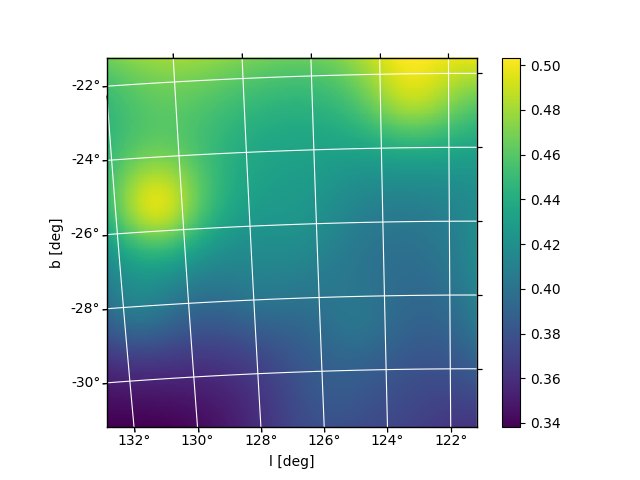
\includegraphics[width=0.49\columnwidth]{figures/mcube_E00_00.png}
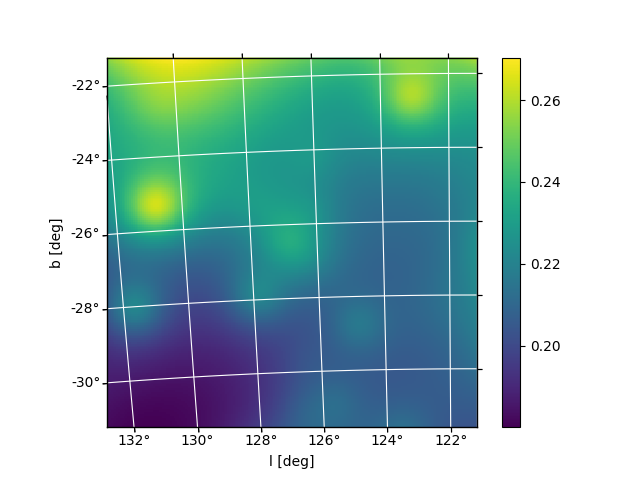
\includegraphics[width=0.49\columnwidth]{figures/mcube_E01_04.png}
\vspace{-0.10in}
\caption{\label{fig:mcube}Model counts maps ($M_{i}$, in counts per $0.05^\circ\times0.05^\circ$ pixel)
  for an example ROI for two energy bins and two different events types. Left, front-converting events 
  from 100~MeV to 133~MeV; right, back-converting events from 316~MeV to 421~MeV.}
\end{centering}
\end{figure}

In words, we define the effective background $B_{ik}$ by
>>>>>>> Stashed changes
convolving $M_{ik}$ with the point-spread function (PSF) at each
energy ($P_k$) and then sum the result over all energies greater than or
equal to a particular energy.

\begin{equation}\label{eq:bkg_eff_defintion}
B_{ik} = \sum_{j \ge k} \frac{M_{ij} \bigotimes P_{j}}{P_{j}^{\rm max}}, 
\end{equation}

\noindent where $P_{j}^{\rm max}$ is the maximum value of the PSF at energy $j$.
Another way of expressing this is that it is the PSF-weighted integral over
the background map.  

The convolution routines in the ScienceTools work on objects of type
{\tt ProjMap} (actually, the sub-classes {\tt HealpixProjMap} and {\tt
  WcsMap2}), which are differential quantities (i.e., they are
intensities, defined at specific energy and directions, rather than
begin integrated across a range of energies and over a pixel.  In
practical terms, this just means that we have to convert the model
counts from either {\tt CountsMap} or {\tt CountsMapHealpix} to a {\tt
  WcsMap2} or {\tt HealpixProjMap}.  We do this just by dividing the
bin contents by the energy bin widths and pixel sizes.

\begin{equation}\label{eq:intensity}
I_{ik} = \frac{M_{ik}}{\delta \Omega_i \delta E_k}.
\end{equation}

\noindent What we actually get back from the PSF convolution routine
is the normalized convolution:

\begin{equation}\label{eq:convolved_intensity}
\tilde{I}_{ik} = I_{ik} \bigotimes P_{k}.
\end{equation}

To get the effective background, we have to convert that quantity back
to counts and sum of all the energy bins greater than or equal to a
particular energy.

\begin{equation}\label{eq:bkg_eff_computation}
B_{ik} = \sum_{j}^{j \ge k} \frac{\tilde{I}_{ij} \delta E_j}{P_{j}^{\rm max}}.
\end{equation}

\noindent Although the factors of $\delta E_k$ in Eq.~\ref{eq:intensity}
and $\delta E_j$ in Eq.~\ref{eq:bkg_eff_computation} cancel, we have 
explicitly kept them in the notation, as they appear in the code because
of the way it is structured.

The quantity $B_{ik}$ has units of counts, and is essentially a counts
map.  We store it as such.  It can be produced by the standalone
application {\tt gteffbkg} or with the {\tt pyLikelihood} interface.
The resulting file will look almost identical to a binned counts map
file, including the {\tt EBOUNDS} and {\tt GTI} HDUs, and the DSS
keywords are copied from the input file.  The only difference will be
the addition of keywords to the primary header of the output file:

\begin{enumerate}
\item{{\tt MAPTYPE} is ``BKG\_EFF''.}
\item{{\tt INPUTMAP} is set to the name of the input binned counts map
file.}
\end{enumerate}

<<<<<<< Updated upstream
=======
Effective background maps at two different energies of our example analysis are shown in 
Fig.~\ref{fig:beff}. 

It is very important to compute the effective background using an ROI 
model that has been padded to account for spill-over from the PSF.  To do this
we first analyzed the ROI without likelihood weights, then used the
script {\tt fermipy-make-wmaps} to correctly make the effective
background maps (and all subsequent steps described below) for an ROI that 
was padded by $5^\circ$ on all sides.

\begin{figure}[h]  
\begin{centering}
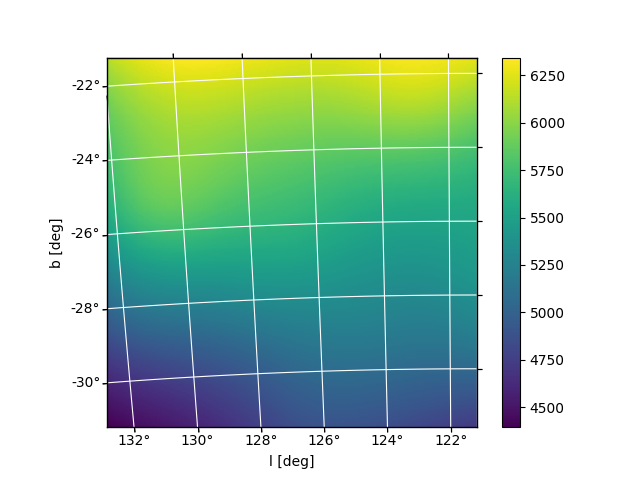
\includegraphics[width=0.49\columnwidth]{figures/beff_E00_00.png}
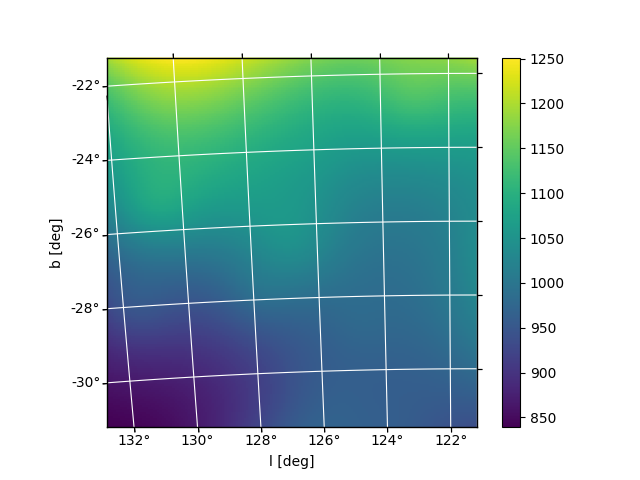
\includegraphics[width=0.49\columnwidth]{figures/beff_E01_04.png}
\vspace{-0.10in}
\caption{\label{fig:beff}Effective background maps ($B_{i}$), in counts per 
  $0.05^\circ\times0.05^\circ$ pixel) for an example ROI
  for two energy bins and two different events types.  Left, front-converting events 
  from 100~MeV to 133~MeV; right, back-converting events from 316~MeV to 421~MeV.}
\end{centering}
\end{figure}



>>>>>>> Stashed changes
\section{The weighted sum over components: \texorpdfstring{$\alpha$}{alpha}}

In order to properly deal with likelihood deweighting for multiple 
data components in one model (e.g., if we are treating 
front-converting and back-converting seperately) we need to
compute the weighted sum over the components.  This quantity depends on
the fractional systematic uncertainty (see \S~\ref{sec:intro})
we are considering ($\epsilon$), on the individual $B_{ikm}$ for each component, and on the
minimum $B_{ikm}$ for the various components for each pixel and energy
bin: $\hat{B}_{ik}$.

We define weight as:

\begin{equation}
\alpha_{ik} = \frac{1 + \epsilon^2 \hat{B}_{ik}}{1 + \epsilon^2 \hat{B}_{ik} \sum_{m} (\frac{\hat{B}_{ik}}{B_{ikm}})^2 }.
\end{equation}

\noindent In the case that we are using a single component, then all
of the $\alpha_{ik} \equiv 1$.

This quantity is dimensionless, and has the same binning as the input
counts map.  It can be produced by the standalone application {\tt gtalphabkg}
or with the {\tt pyLikelihood} interface.  This will store almost
exactly the same information as a {\tt CountsMap} or {\tt
  CountsMapHealpix}. Since we are using several components, we remove 
the DSS keywords.  However we do add some keywords specifying the
provenance of the map:

\begin{enumerate}
\item{{\tt MAPTYPE} is ``ALPHA\_BKG'';}
\item{{\tt EPSILON}: has the value of $\epsilon$ used in the computation;}
\item{{\tt BKGMAPXX}: lists the input effective background maps.}    
\end{enumerate}

<<<<<<< Updated upstream
=======
Maps of the parameter $\alpha_{ik}$ for our example analysis are shown in Fig.~\ref{fig:alpha}.

\begin{figure}[h]  
\begin{centering}
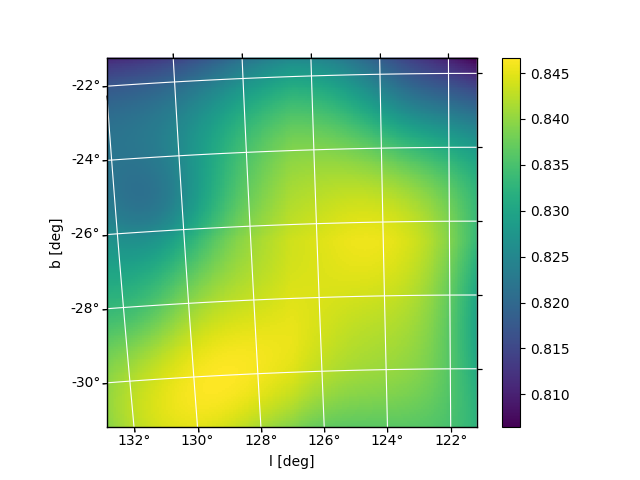
\includegraphics[width=0.49\columnwidth]{figures/alpha_E00_00.png}
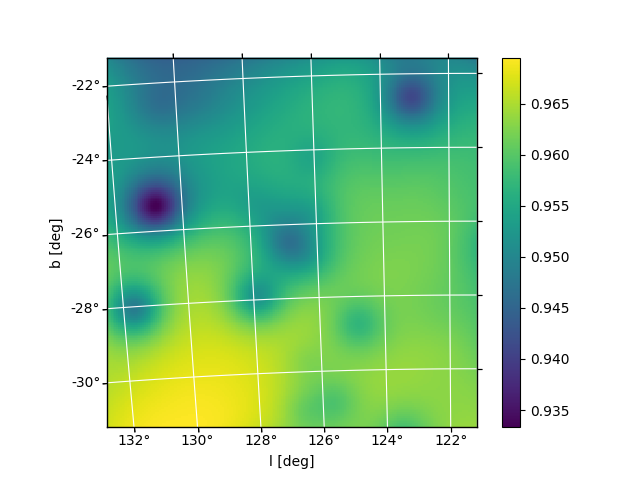
\includegraphics[width=0.49\columnwidth]{figures/alpha_E01_04.png}
\vspace{-0.10in}
\caption{\label{fig:alpha}Maps of $\alpha_{i}$ for our example ROI
  for two energy bins, obtained by combining front-converting and 
  back-converting events and setting the systematic error level
  to $\epsilon = 0.03$.  Left, 100~MeV to 133~MeV; right 316~MeV to 421~MeV.}
\end{centering}
\end{figure}


\section{Choosing the value of the fractional systematic uncertainty}

The {$\it Fermi$}-LAT collaboration arrived at a value of $\epsilon = 0.03$ by 
picking a value so that the standard deviation of the uncertainty-scaled residuals 
of the energy flux for individual energy bins for a large number of spectral fits 
was close to one.  Put another way, we picked $\epsilon = 0.03$ because that value
re-scaled the errors of SED measurements to give a $\chi^2$ per degree of freedom 
close to one.
>>>>>>> Stashed changes


\section{The likelihood weights: \texorpdfstring{$w$}{w}}

Given the effective background maps and the $\alpha_{ik}$, the
likelihood weights for a particular component are defined as:

\begin{equation}
w_{ikm} = \frac{\alpha_{ik}}{1 + \epsilon^2 B_{ikm}}.
\end{equation}

This quantity is dimensionless and has the same binning as the input
counts map.  It can be produced by the standalone application {\tt gtwtsmap}
or with the {\tt pyLikelihood} interface.  However, for
historical reasons, the {\tt BinnedLikelihood} object expects the
weights to be given as an object of the class {\tt ProjMap}.  In the
{\tt fermitools} {\tt ProjMap} objects usually represent intensity maps,
but there is nothing enforcing this.  In practical terms the only real
difference for a weights file is that it is defined at specific
energies rather than over energy ranges.  This means that we replace
the {\tt EBOUNDS} HDU with an {\tt ENERGIES} HDU.

Aside from that, the $w_{ik}$ files have almost exactly the
same information as a {\tt CountsMap} or {\tt CountsMapHealpix},
including the DSS keywords copied from the file with the $B_ik$; the
only differences being the additional keywords:

\begin{enumerate}
\item{{\tt MAPTYPE} is ``WEIGHT\_MAP''.}
\item{{\tt EPSILON}: has the value of $\epsilon$ used in the computation;}
\item{{\tt BKGMAP}: has the name of the file with the input effective background map.}    
\item{{\tt ALPHAMAP}: has the name of the file containing the input $\alpha$ map (if used).}
\end{enumerate}


\section{Using the likelihood weights.}

The idea is that using the likelihood weights is almost transparent.
If a likelihood weights map is specified when the {\tt BinnedLikelihood}
object is being created, those weights will be used; otherwise no
weights will be used.

Depending on the interface used, the likelihood weights can be
specified in a number of ways.

\begin{enumerate}
\item{By passing an object of type {\tt ProjMap} (actually either a
    {\tt WcsMap2} or a {\tt HealpixProjMap}) into the constructor of
    {\tt BinnedLikelihood}.  The map will be re-sampled, taking the
    coordinate information from the bin and pixel centers of the {\tt CountsMapBase}
    and requesting the {\tt ProjMap} value for those.}
\item{By passing a file name into the constructor of {\tt
      pyLikelihood.BinnedAnalysis}.  This points to any file that
    contains a valid {\tt ProjMap}, and the file will be 
    resampled as above.}
\item{By specifying a file name for the hidden {\tt wmap} parameter of
    {\tt gtlike} or {\tt gtscrmaps}.  This points to any file that
    contains a valid {\tt ProjMap}, and the file will be 
    resampled as above.}
\end{enumerate}

<<<<<<< Updated upstream
=======

\section{Effect of using the likelihood weights.}

Since the likelihood weights are constructed to be less than one, they 
have the effect of reducing the likelihood, and also reducing changes in 
the likelihood.  Since uncertainty estimates and upper limits are defined
in terms of changes in the likelihood, using the likelihood weights 
will result in larger uncertainties and higher upper limits.  

The effect on fits to the normalization of 4FGL J0047.9+3947 
for the lowest energy bin in our example analysis is shown in Fig.~\ref{fig:ll}.

\begin{figure}[h]  
\begin{centering}
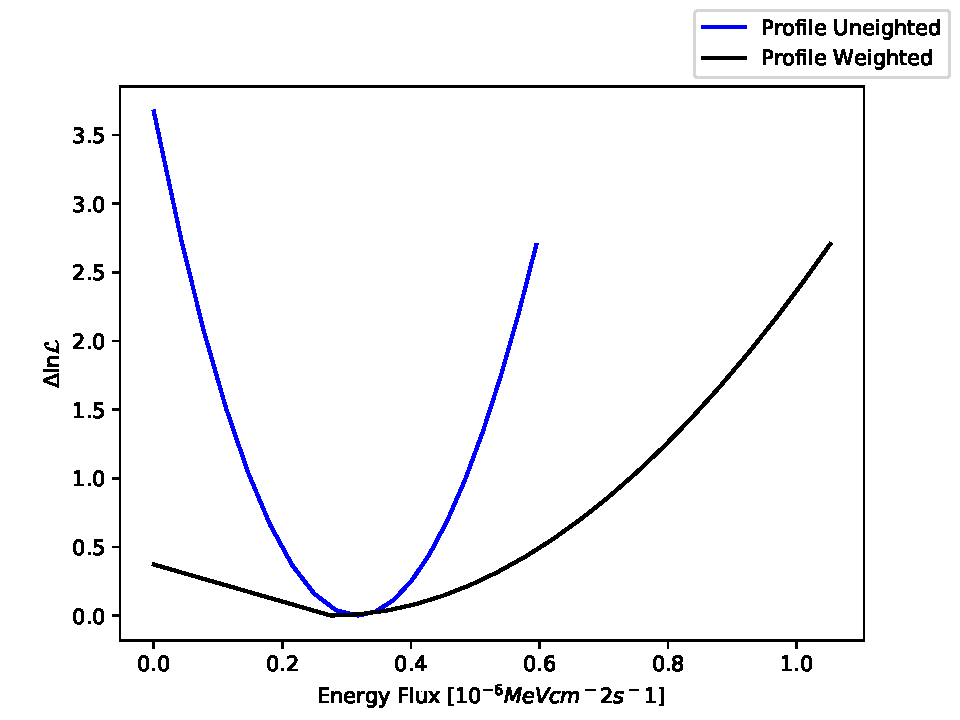
\includegraphics[width=\columnwidth]{figures/ll_compare.pdf}
\vspace{-0.10in}
\caption{\label{fig:ll}Change in profile log likelihood ($\Delta\log\mathcal{L}$ with 
  respect to the best-fit value) for 4FGL J0047.9+3947 as a function of the 
  normalization in the energy range 100~MeV to 133~MeV.}
\end{centering}
\end{figure}

The effect on fitting the spectral energy density (SED) of a point 
source in our example analysis is shown in Fig.~\ref{fig:sed}.  Clearly 
the effect of the likelihood weighting is largest for the lower energy bins, 
where the effective background is larger and the
weights are smaller.

\begin{figure}[h]  
\begin{centering}
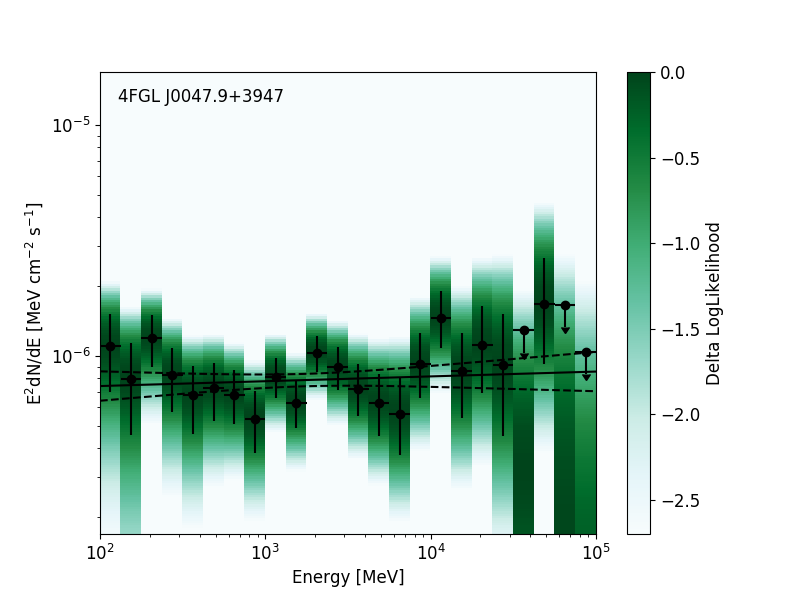
\includegraphics[width=0.49\columnwidth]{figures/sed_nowts.png}
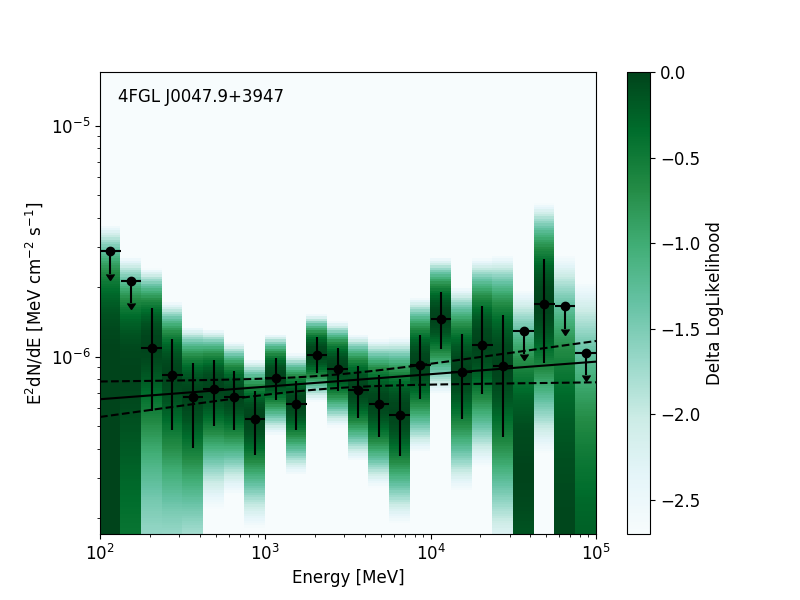
\includegraphics[width=0.49\columnwidth]{figures/sed_wts.png}
\vspace{-0.10in}
\caption{\label{fig:sed}SED of 4FGL J0047.9+3947, including the $\Delta\ln\mathcal{L}$ shown
  with the under-laid color scale. Results
  for the un-weighted (weighted) likelihood are shown on the left (right).}
\end{centering}
\end{figure}]


\section{Acknowledgments}

This implementation and equations are based on 
Jean Ballet's work.\footnote{Extensive notes can be found at: \url{https://confluence.slac.stanford.edu/x/ZphdCw}}

>>>>>>> Stashed changes
\end{document}
 

% LocalWords:  ScienceTools ROI convolving PSF ProjMap HealpixProjMap WcsMap2
% LocalWords:  CountsMap CountsMapHealpix gteffbkg pyLikelihood EBOUNDS GTI DSS
% LocalWords:  HDUs MAPTYPE BKG INPUTMAP gtalphabkg BKGMAPXX gtwtsmap HDU wmap
% LocalWords:  BinnedLikelihood BKGMAP ALPHAMAP CountsMapBase BinnedAnalysis Eq
<<<<<<< Updated upstream
% LocalWords:  gtlike gtscrmaps
=======
% LocalWords:  gtlike gtscrmaps fermitools Laboratoire CEA IRFU Astrophysique
% LocalWords:  Saclay Gif sur mis LATs de fermipy MeV GeV P8R3 SOURCE J0047
% LocalWords:  V2 gll iem v07 4FGL v1 txt iso SED un wmaps
>>>>>>> Stashed changes
